\documentclass{article}
\usepackage[utf8]{inputenc}
\usepackage[left=2cm,top=2.5cm,right=2cm,bottom=2.5cm]{geometry} 
\usepackage[spanish]{babel}
\usepackage{graphicx} 
\usepackage{placeins}
\usepackage{makeidx}
\usepackage{multirow, array}
\usepackage{float}

\title{Primera entrega proyecto OI}
\date{28 de mayo de 2017}

\begin{document}

\maketitle
\begin{abstract}

El precio del combustible uruguayo es el más caro de la región*. ANCAP regula tanto el precio intermedio como el final de los combustibles. La bonificación que obtienen las 447 estaciones de servicio (EESS) a lo largo del país se desprende de la paramétrica, esta pretende reflejar la estructura de costos de una estación tipo. La estación tipo se construyó a partir de una muestra aparentemente representativa de 52 EESS y sus respectivas estructuras de costos, no obstante, la estación tipo no se derivó directamente de la muestra sino luego de negociaciones entre la UNVENU (Unión de Vendedores de Nafta de Uruguay) y ANCAP. Intuitivamente la construcción de una paramétrica a partir de una estación tipo parece problemática por la heterogeneidad en la estructura de costos que se puede imaginar, estas presentan según sus propias características. A su vez, no está claramente definido cada cuánto se actualiza la paramétrica ni hay un protocolo definido si existen discrepancias entre la evolución de las variables que constituyen a la paramétrica y la paramétrica per se. De hecho, la paramétrica no se ha actualizado desde mediados del año pasado donde hubo un ajuste de los salarios de la rama. A fines del año 2016 desde ANCAP se propusieron dos medidas: i) construir tres franjas de bonificaciones según el ‘litraje’ vendido; ii) desregular el precio final de los combustibles. Es pertinente destacar que la desregulación del precio final presenta posibles problemáticas entre ellas: la integración vertical. DUCSA, distribuidora privada, propiedad de ANCAP, posee 2 EESS y a su vez, la propiedad de varias de estas. Pretendemos aportar evidencia para una discusión más rigurosa sobre si mejorar la regulación del sistema de bonificaciones que perciben las EESS o alternativamente, proponer un sistema que se aproxime a la desregulación del precio.
\end{abstract}

*\begin{figure}[H]
\caption{Precio en dólares por litro del combustible para países de América}
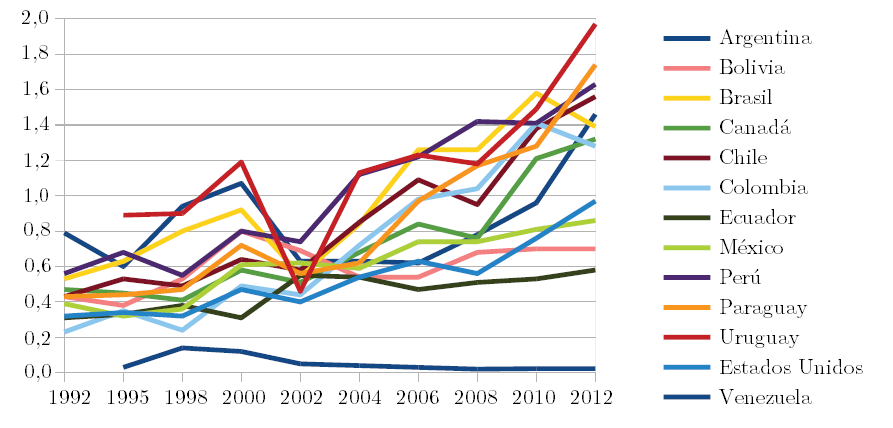
\includegraphics[width=0.6\textwidth]{pum.png}
\end{figure}
\FloatBarrier 
\noindent\textbf{Fuente:} Domingo, R.; Zipitría, L. (2015). Regulación de empresas públicas en Uruguay desafíos y perspectivas.\newline

\begin{table}[ht]
\caption{Precio en dólares por litro del combustible (al 22/05/2017) para países de América} 
\resizebox{17cm}{!} {
\begin{tabular}{c c c c c c c c c c c c c} % centered columns (4 columns)
\hline\hline %inserts double horizontal lines
Argentina & Bolivia & Brasil & Canadá & Chile & Colombia & Ecuador & Estados Unidos & México & Perú & Paraguay & Uruguay & Venezuela \\ [0.5ex] % inserts table
%heading
\hline % inserts single horizontal line
1.21 & 0.52 & 1.14 & 0.91 & 1.14 & 0.74 & 0.39 & 0.70 & 0.93 & 0.98 & 0.98 & 1.59 & 0.01 \\ [1ex] % [1ex] adds vertical space
\hline %inserts single line
\end{tabular}%
}
\label{table:nonlin} % is used to refer this table in the text
\end{table}
\FloatBarrier 
\noindent\textbf{Fuente:} http://www.globalpetrolprices.com/gasoline\_prices/\newline
\end{document}
